\documentclass[11pt,a4paper]{book}
\usepackage{amsmath}
\usepackage[dutch]{babel}
\usepackage{graphicx}
\usepackage{picture}
\usepackage{color}
\usepackage{graphpap,color}
\usepackage{subfig}
\usepackage[percent]{overpic}

\usepackage[dutch]{babel}
\usepackage{amsfonts}
\usepackage{amssymb}
\usepackage{makeidx}
\usepackage{pdflscape}
%\usepackage{booktabs}
%\usepackage[usenames,dvipsnames,svgnames,table]{xcolor}
\definecolor{kuleuven}{RGB}{29,141,176}
\definecolor{kuleuven1}{RGB}{82,189,236}
\usepackage{geometry}

\newcommand{\nocontentsline}[3]{}
\newcommand{\tocless}[2]{\bgroup\let\addcontentsline=\nocontentsline#1{#2}\egroup}



\makeindex
\begin{document}
\renewcommand*\chaptername{Hoofdstuk}
\renewcommand*\bibname{Bibliografie}
\renewcommand*\appendixname{Bijlagen}

\frontmatter
\newgeometry{textwidth=540pt,textheight=780pt,top=20pt,left=20pt,right=20pt}
\begin{titlepage}

\begin{figure}[tc]{%
      \begin{overpic}[width=1\textwidth,natwidth=50,natheight=0]{img/Picture1.png}
        \put(35,4){\color{white}{\textbf{FACULTEIT ECONOMIE EN BEDRIJFSWETENSCHAPPEN}}}
      \end{overpic}
    }
\end{figure}

\vspace*{4.5cm}
{\color{kuleuven1}{\Huge Identification of important contributions in diagnostic medical imaging}}

\vspace*{0.5cm}
{\Large Identificatie van belangrijke contributies in diagnostische medische beeldvorming}

\begin{figure}[bl]
  %\centering
   \begin{minipage}[c]{0.4\textwidth}  {%
      \begin{overpic}[width=0.9\textwidth,natwidth=300,natheight=370]{img/Picture2.png}
        \put(70,45){\begin{minipage}[c]{1.80\textwidth}
\begin{flushright}

{\Large Ir. Sven Van Hove} \linebreak
{s0190440} \linebreak
   
\textbf{{\large Masterproef aangeboden tot  \linebreak
het behalen van de graad}} \linebreak
\linebreak
{\large \textsc{Master in het Management}}\linebreak
{\large }\linebreak
\linebreak
\textbf{{\large Promotor:}}  Prof. Dr. R. Veugelers \linebreak
\textbf{{\large Werkleider:}} D. Verhoeven
\linebreak

\textbf{{\large Academiejaar}} {\large 2013-2014}
\linebreak
\end{flushright}
  \end{minipage}}
      \end{overpic}
    }
  \end{minipage}
  
  
\begin{picture}(540,0.2)
\put(0,0){\colorbox{kuleuven1}{\makebox(540,0.2){}}}
\end{picture}
\end{figure}

\end{titlepage}
%%%%%%%%%%%%%%%%%%%%%%%%%%%%%%%%%%%%%%%%%%%%%%%%%%%%%%%%%%%%%%%%%%%%%%%%%%%%%%%%%%%%%%%%%%%%%%%%%%%%
\restoregeometry
\setcounter{equation}{1}

\pagestyle{empty}

\renewcommand*\contentsname{Inhoud}
\tableofcontents

%%%%%%%%%%%%%%%%%%%%%%%%%%%%%%%%%%%%%%%%%%%%%%%%%%%%%%%%%%%%%%%%%%%%%%%%%%%%%%%%%%%%%%%%%%%%%%%%%%%%%%%%%

%\chapter*{Abstract\hfill}\addcontentsline{toc}{chapter}{Abstract}

\cleardoublepage
\thispagestyle{plain}
\begin{center}
    \Huge 
    Identification of important contributions in diagnostic medical imaging
    
    \vspace{0.5cm}
    
    \large
    Identificatie van belangrijke contributies in diagnostische medische beeldvorming
    
    \vspace{1.0cm}
    
    Sven Van Hove, Dennis Verhoeven, Reinhilde Veugelers
    
    \vspace{0.5cm}
    
	Managerial Economics, Strategy and Innovation (MSI)\\
	Faculteit Economie en Bedrijfswetenschappen\\
	KU Leuven
    
    \vspace{1.0cm}
    \textbf{Abstract}
\end{center}

Radical innovations have the power to disrupt whole technological fields, and
are often seen as a key factor in long term growth. Therefore it is critical to
identify early on how radical an innovation is. In this thesis, we performed a
manual assessment of five interesting innovations in the field of diagnostic medical
imaging: digital radiography, electron beam computed tomography, magnetic
resonance imaging, 18F-FDG tracers in nuclear medicine and the application of
computer aided detection and diagnosis in mammography. The assessment was
performed based on a framework proposed by \cite{verhoeven}. This framework
contains three dimensions: novelty of knowledge origins, novelty of
functionality  and technological impact. The resulting scores turned out lower
than expected, so we looked into possible causes. In the future these scores can
be compared against the outcome of an automatic assessment based on patent
indicators. Conclusions drawn from this comparison could be used to optimize the
framework.

\vspace{1.0cm}

\textbf{Keywords:} important technological inventions, radical innovation,
diagnostic medical imaging, manual assessment, patent indicators. %TODO dankwoord?
\mainmatter
\pagestyle{headings}

\chapter{Inleiding}
\section{Situering}
\begin{itemize}
  \item context: FEB, strategie
  \item radiacale innovatie
  \item diagnostische medische beeldvorming
\end{itemize}


\section{Methodologie}
\begin{itemize}
  \item veld afbakenen
  \item innovaties zoeken + score
  \item validatie a.h.v. papers
\end{itemize}

\section{Vervolg van deze tekst}

%Beschrijving van uitvindingen

%Score per uitvinding

%Resultaten

\chapter{Conclusie}

\clearpage %clearbothpages?
\bibliographystyle{alpha} %plain,unsrt,alpha,abbrv,acm,apalike,siam,ieeetr,..
\bibliography{references} \addcontentsline{toc}{chapter}{Bibliografie}

\vfill

\appendix
\begin{landscape}
	\chapter{Assessment sheet}\label{app:score}
	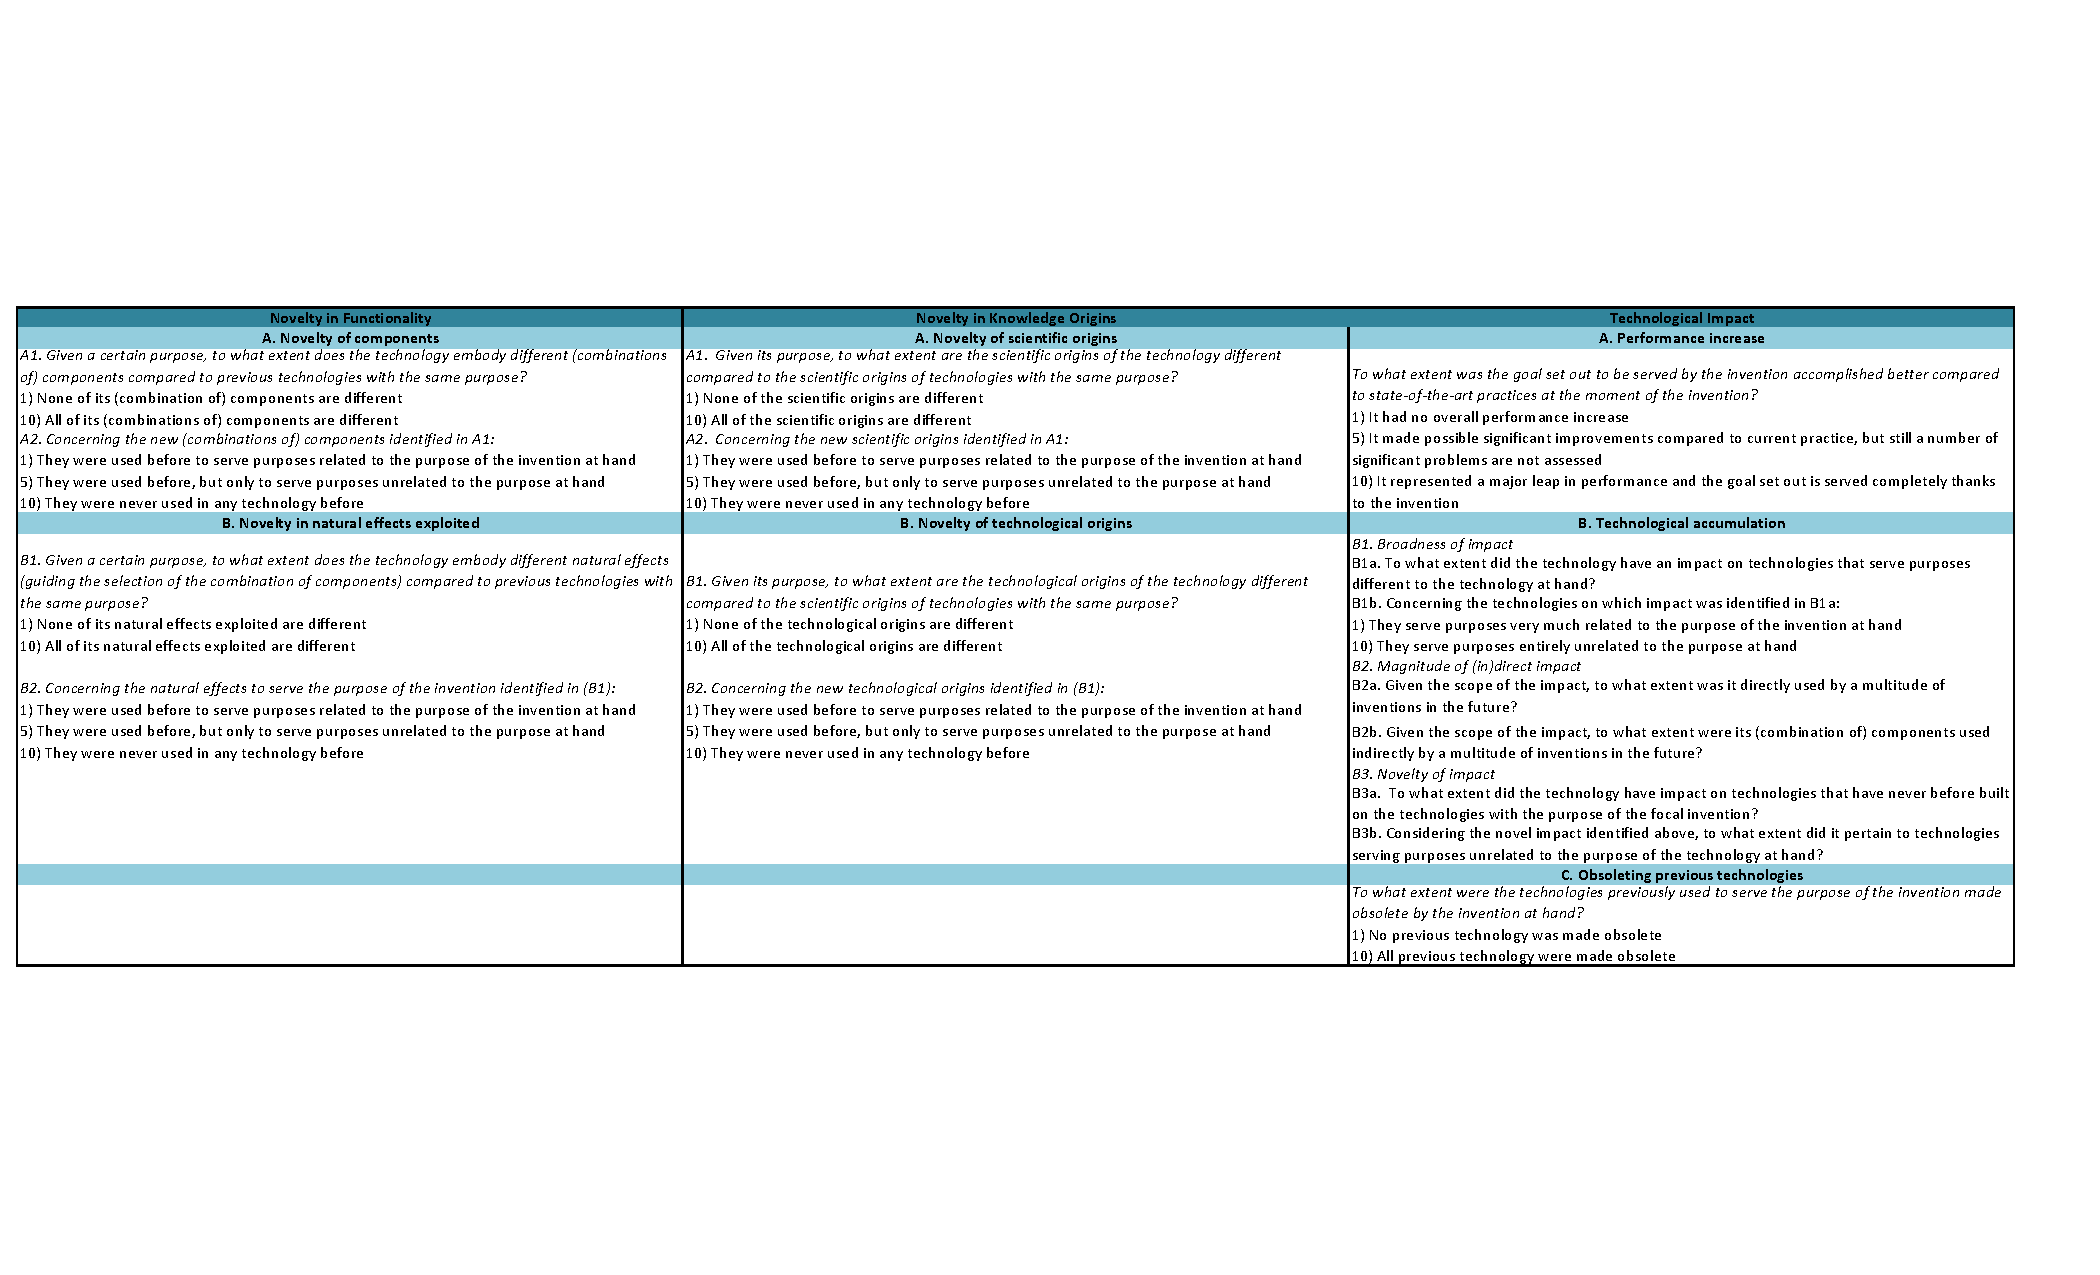
\includegraphics[width=1.0\linewidth, trim=5 150 60 150]{img/score.pdf}
\end{landscape}

\chapter{International Patent Classification codes}
This section contains a list of relevant patent categories in relation to
diagnostic medical imaging. The categories are identified using their
International Patent Classification (IPC) codes. A complete reference of all IPC
codes can be found at \url{http://web2.wipo.int/ipcpub}.

\begin{description}
  \item[A61B 1/005] Flexible endoscopes
  \item[A61B 5/05] Measuring for diagnosis by means of electric currents or magnetic fields
  \item[A61B 6/00] Apparatus for radiation diagnosis, e.g. combined with radiation therapy equipment
  \item[A61B 6/03] Computerised tomographs
  \item[A61B 8/00] Diagnosis using ultrasonic, sonic or infrasonic waves
  \item[G01N 23/00] Investigating or analysing materials by the use of wave or particle radiation
  \item[G01R 33/00] Arrangements or instruments for measuring magnetic variables
  \item[G01T 1/36] Measuring spectral distribution of X-rays or of nuclear radiation
  \item[G01T 1/161] Applications in the field of nuclear medicine, e.g. in vivo counting
  \item[G02B 23/24] Instruments for viewing the inside of hollow bodies, e.g. fibrescopes
  \item[G03B 42/02] using X-rays
  \item[G06T] IMAGE DATA PROCESSING OR GENERATION, IN GENERAL 
  \item[H01J 35/00] X-ray tubes
  \item[H05G] X-RAY TECHNIQUE
\end{description}

\newpage
\thispagestyle{empty}
\newgeometry{textwidth=540pt,textheight=780pt,top=20pt,left=20pt,right=20pt}
\begin{figure}[ht]
\begin{flushright}
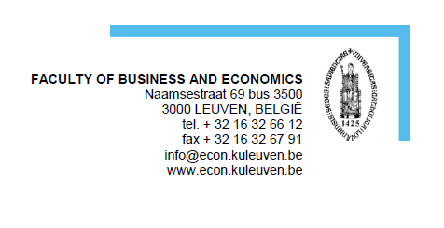
\includegraphics[width=0.5\textwidth,natwidth=310,natheight=10]{img/Picture3.png}	
\end{flushright}
\end{figure}
\vfill
\begin{picture}(550,40)
\put(0,0){\colorbox{kuleuven}{\makebox(520,52){}}}
\end{picture}
\end{document}